The proposed solution of the steady-state dynamic temperature estimation can be used in a wide range of optimization procedures. One of them is the reliability optimization that we discuss in this section. We performing the temperature-aware task mapping and scheduling in order to address the thermal cycling aging effect while keeping the energy consumption on an appropriate level. Both mapping and scheduling are based on the genetic algorithms \cite{schmitz2004}. Let us start with the overall description of the system.

\subsection{Application Model}
The system executes a periodic application with a set of data-dependent tasks. The overall structure of the application is defined by a task graph:
\begin{align*}
  & G = (\mathcal{V}, \: E, \: \mathcal{T}) \\
  & \mathcal{V} = \{ v_i \} \\
  & E = \{ e_{ij} \}
\end{align*}
where $\mathcal{V}$ is a set of $N_t$ vertices of the graph (tasks), $E$ is a set of edges (data dependencies between tasks), and $\mathcal{T}$ is the period of the application. Each pair of a task $v_i$ and a processing element $\pi_k$ is characterized by two parameters:
\begin{equation*}
  (v_i, \pi_k) \rightarrow (C_{eff \; ik}, N_{cycles \; ik})
\end{equation*}
where $C_{eff \; ik}$ is the effective switched capacitance and $N_{cycles \: ik}$ is the number of clock cycles. These parameters determine the processor load and execution time of the task, correspondingly.

\subsection{Temperature-Aware Reliability Model}
In the paper we address temperature-driven failure mechanisms with the reliability model presented in \cite{huang2009}, \cite{xiang2010}. The model is based on the assumption that the failure rate has a Weibull distribution (e.g., the thermal cycling, electromigration, etc. \cite{jedec2010}):
\[
  R(t) = e^{-(\frac{t}{\eta})^\beta}
\]
where $\eta$ is the scaling parameter, $\beta$ is the shape (slope) parameter. The mean time to failure (MTTF) for the Weibull distribution is given by the following equation:
\begin{equation} \label{eq:general-mttf}
  MTTF = \eta \; \Gamma(1 + \frac{1}{\beta})
\end{equation}
where $\Gamma$ is the gamma function. The shape parameter is found to be independent on the temperature variation \cite{chang2006}, which is not the case with the scaling parameter $\eta$. Therefore, the distribution can vary from one set of conditions to another. We can use the same approach as it was shown previously and split the overall period of the application $\mathcal{T}$ into $N_m$ time intervals $\triangle t_i$, so that during each time interval $\triangle t_i$ all those conditions can be treated as constants, consequently, the corresponding $\eta_i$ is also constant. In this case, the cumulative distribution function by the end of the first execution of the application is the following \cite{huang2009}, \cite{xiang2010}:
\[
  R = e^{-(\sum_{i=0}^{N_m - 1} \frac{\triangle t_i}{\eta_i})^\beta}
\]

It can be shown that if $\eta_i$ are large enough\footnote{This is the case, since usually the MTTF is in order of tens of years (see \equref{eq:general-mttf}).}, the following continuous approximation can be applied \cite{xiang2010}:
\[
  R(t) = e^{-(\frac{t}{\mathcal{T}} \sum_{i=0}^{N_m - 1} \frac{\triangle t_i}{\eta_i})^\beta}
\]
The formula still keeps the form of the Weibull distribution with the following scaling parameter:
\[
  \eta = \frac{\mathcal{T}}{\sum_{i=0}^{N_m - 1} \frac{\triangle t_i}{\eta_i}}
\]

As it was mentioned earlier, the reliability model can be used to model different failure mechanisms. Let us now focus on one particular failure cause, the thermal cycling (TC) fatigue, that is a common packaging and interfacial failure mechanism \cite{jedec2010}. The number of cycles to failure can be estimated using a modified version of the well-known Coffin-Manson equation with the Arrhenius term \cite{jedec2010}, \cite{xiang2010}, \cite{ciappa2003}:
\begin{equation} \label{eq:cycles-to-failure}
  \mathcal{N} = A (\triangle T - \triangle T_0)^{-b} e^{\frac{E_a}{k T_{max}}}
\end{equation}
where $A$ is an empirically determined constant, $\triangle T$ is the thermal cycle amplitude, $\triangle T_0$ is the portion of the temperature range in the elastic region which does not cause damage, $b$ is the Coffin-Manson exponent which also empirically determined\footnote{This constant is found to be 6--9 for brittle fracture such as Si and its dielectrics \cite{jedec2010}.}, $E_{a}$ is the activation energy\footnote{For the thermal cycling failure mechanism the activation energy lies between 0.5 and 0.7~eV \cite{vigrass}.}, $k$ is the Boltzmann constant, and $T_{max}$ is the maximal temperature during the thermal cycle. Having the number of cycles to failure and the duration of one cycle $\triangle t$, we can compute the MTTF:
\[
  MTTF = \mathcal{N} \; \triangle t
\]

Since we consider the TC failure mechanism, the time intervals $\triangle t_i$ correspond to intervals of constant parameters of this particular mechanism that can be observed on \equref{eq:cycles-to-failure}. Each interval $\triangle t_i$ belongs to one thermal cycle with the scaling parameter $\eta_i$ derived using \equref{eq:general-mttf}:
\[
  \eta_i = \frac{MTTF_i}{\Gamma(1 + \frac{1}{\beta})}
\]
where $MTTF_i$ is the mean time to failure of the $i$th time interval as if we had the failure distribution of this interval all the time. Taking everything together, we get the following equation:
\begin{equation} \label{eq:one-mttf}
  MTTF = \frac{\mathcal{T}}{\sum_{i=0}^{N_m - 1} \frac{1}{\mathcal{N}_i}}
\end{equation}

\equref{eq:one-mttf} describes the MTTF of one component, which is a processing element in our case. We assume that \emph{each} processing element is essential for the proper work of the system, therefore, a failure of \emph{any} core leads to the total failure of the whole system. Consequently, the MTTF of the system can be estimated as the minimal MTTF among its components:
\begin{align*}
  & MTTF_{sys} = \min_{k=0}^{N_p - 1} \; MTTF_k \\
  & MTTF_k = \frac{\mathcal{T}}{\sum_{i=0}^{N_{mk} - 1} \frac{1}{\mathcal{N}_{ik}}}
\end{align*}
where $N_{mk}$ is the number of thermal cycles of the $k$th processing element within the application period $\mathcal{T}$ and $\mathcal{N}_{ik}$ is the number of thermal cycles to failure if the $i$th cycle was repeated all the time.

\subsection{Motivational Example} \label{sec:motivation}
Consider an application with six tasks, denoted ``T0''--``T5'', and a heterogeneous architecture with two cores, labeled ``PE0'' and ``PE1''. The task graph of the application is given in \figref{fig:task-graph} along with the execution times for both cores. The period of the application is 0.06 seconds. A first alternative mapping and schedule, and the resulting SSDTP are shown at the top of \figref{fig:motivation} (where the hight of a task represents its relative dynamic power consumption). It can be observed that initially PE0 is experiencing three thermal cycles. If we change the mapping of T5 and move it to PE1, we achieve two thermal cycles of PE0 instead of three. Finally, if we vary the schedule as well and change the order of T1 and T3, the number of cycles of PE0 becomes one. Using the reliability model from \secref{sec:reliability-model}, we observe improvements in the MTTF of 44.69\% and 54.53\%, respectively, relative to the initial configuration.
\begin{figure}
  \centering
  \subfloat[The task graph.]{
    \label{fig:task-graph}
    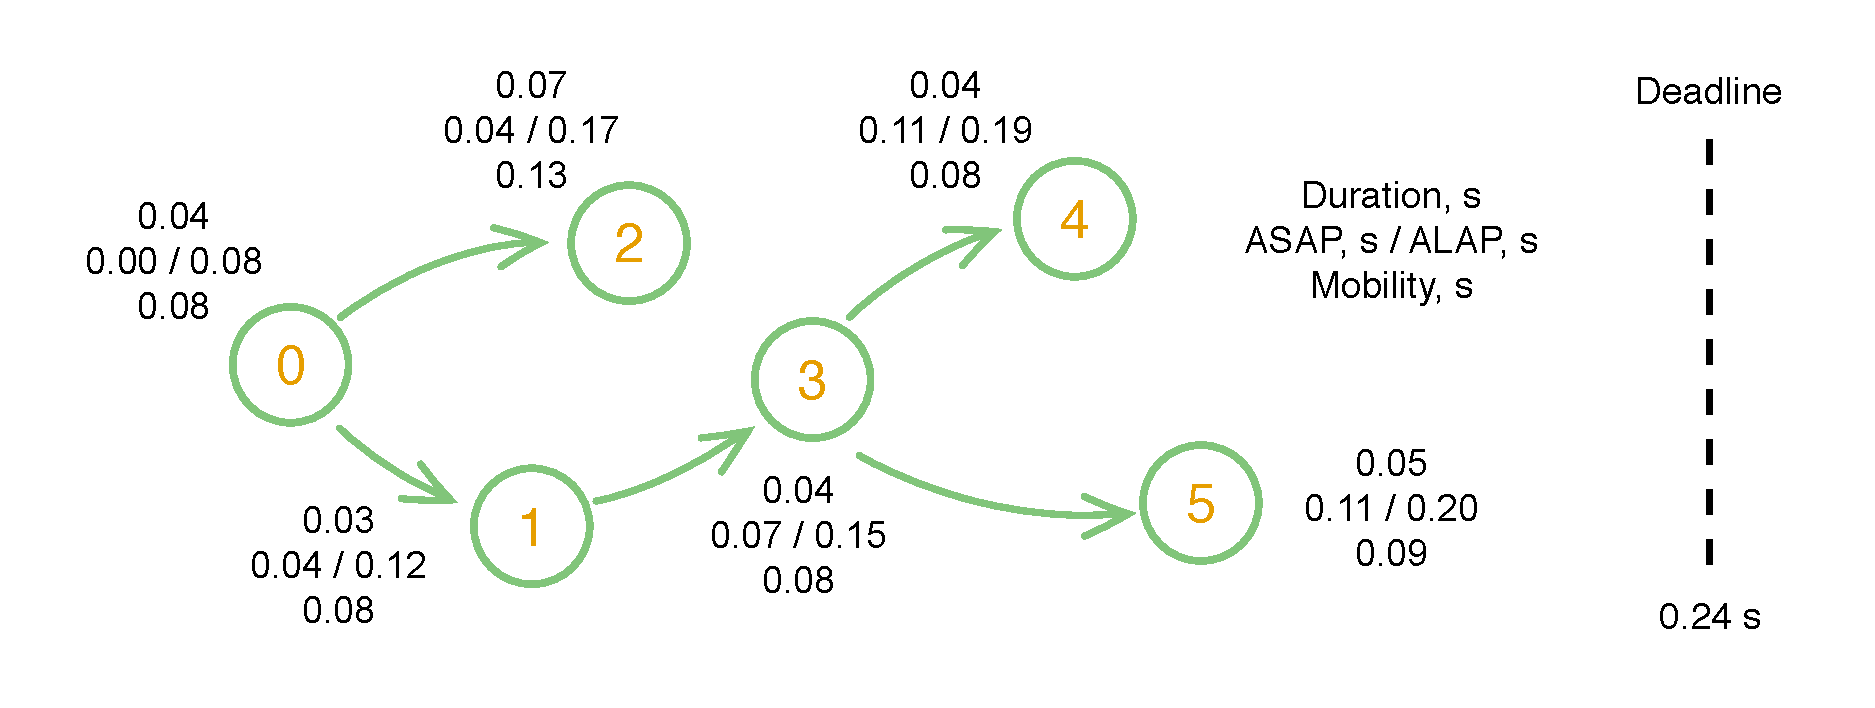
\includegraphics[width=0.8\linewidth]{assets/task-graph.pdf}
  }
  \vspace{-15pt}

  \subfloat[Alternative mappings and schedules.]{
    \label{fig:motivation}
    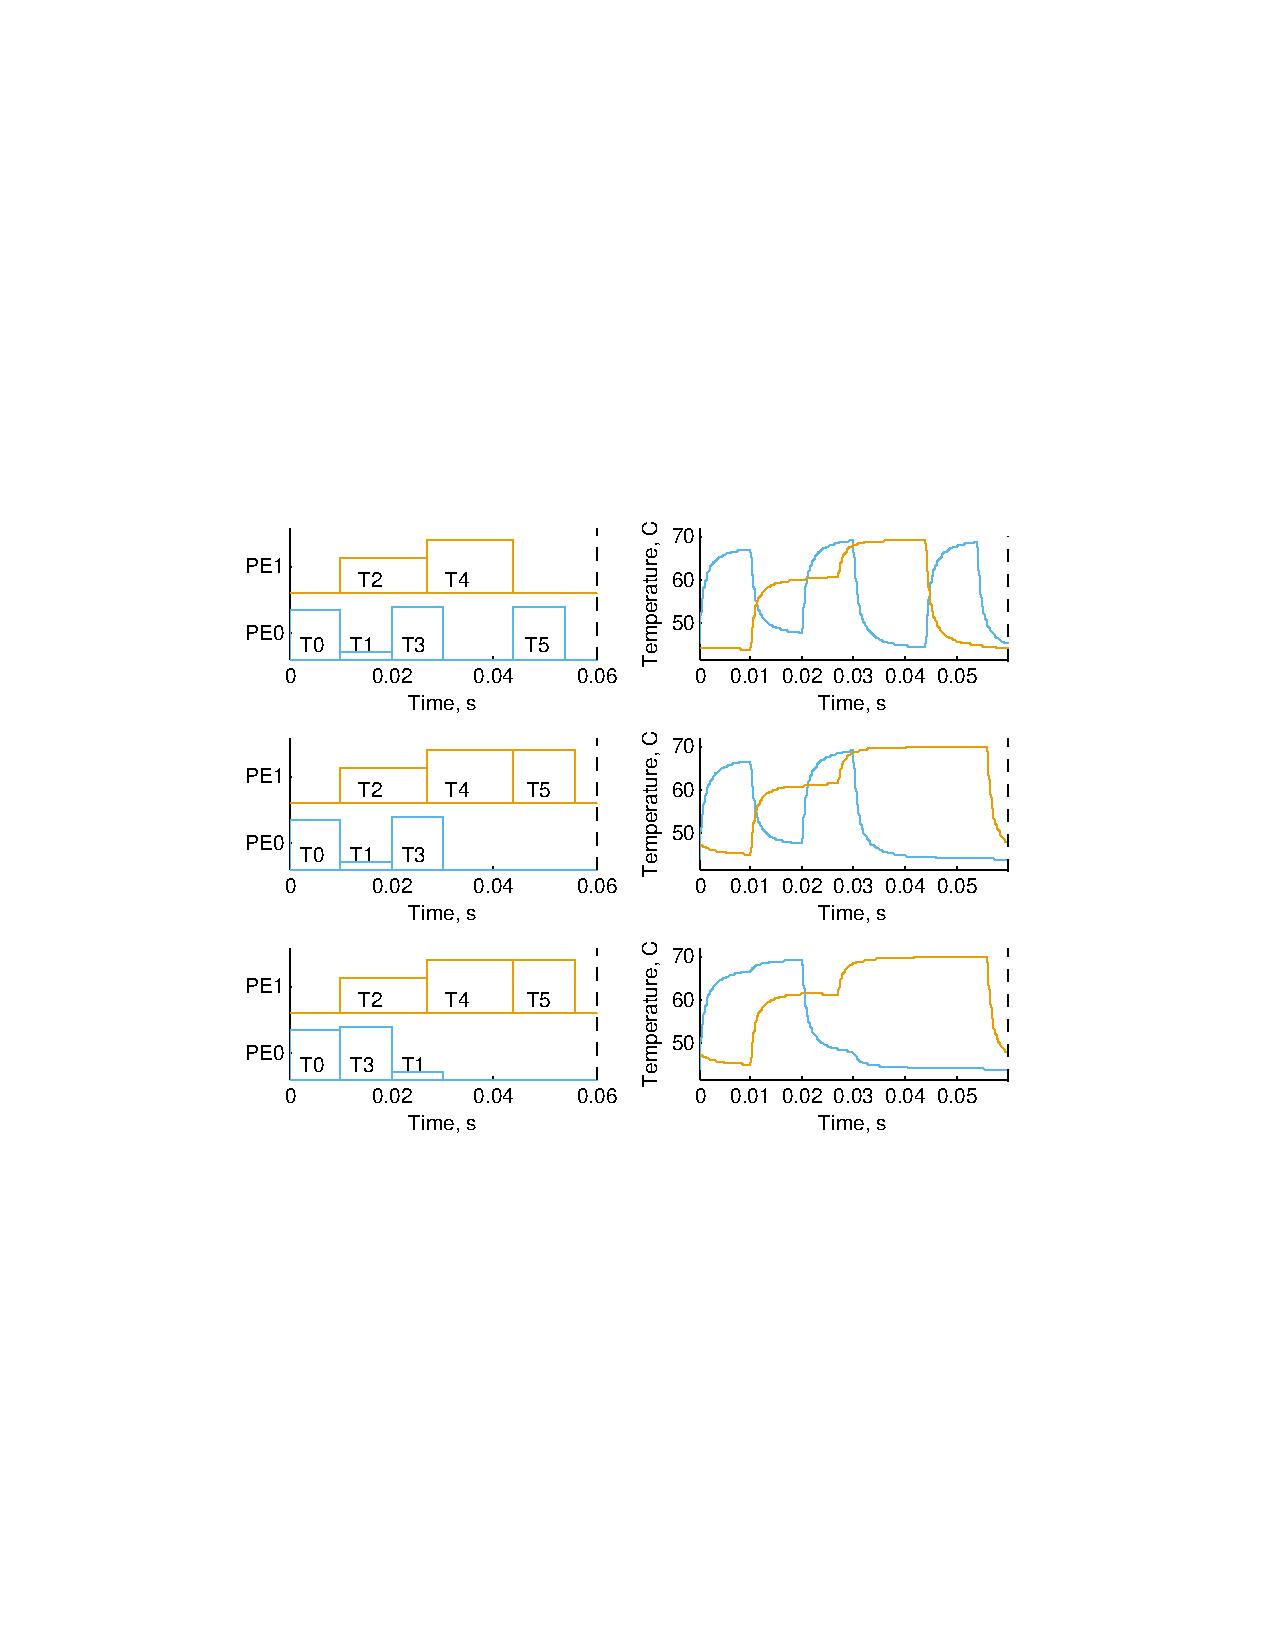
\includegraphics[width=0.8\linewidth]{assets/motivation.pdf}
  }
  \vspace{5pt}
  \caption{Motivational example.}
  \vspace{15pt}
\end{figure}


\subsection{Genetic Algorithm}
TO BE DONE.
